\section{Introduction}
Language Models (LMs) are maturing into powerful tools for scientific discovery~\citep{karpathy2026autoresearch}. Early milestones are striking, from virtual LM teams designing SARS-CoV-2 nanobody binders~\citep{swanson2025virtual} to models proposing NLP research directions that human experts rate as genuinely novel~\citep{si2024can}. However, these successes rely heavily on prompting existing frontier models that are extensively pre-trained on massive corpora of text. In contrast, human scientists achieve breakthroughs through a far more efficient process: by synthesizing profound insights from sparse and disparate sources. Emulating this human-like capability of conjecturing is not just a theoretical ideal; it is a practical necessity as LMs struggle to reliably generate ideas of true impact and value~\citep{si2025ideation}, often due to the lack of diversity and feasibility~\citep{wadhwa2026createtestingllmsassociative}. 

To bridge this gap, we propose a new paradigm: \emph{insight anticipation}. Rather than focusing on broad data assimilation, this setting tasks models with predicting the natural evolutionary trajectory of specific, existing research. This framing adopts the classical view of scientific progress as `\emph{standing on the shoulders of giants,}' where new contributions emerge by building incrementally upon prior foundations. Under this view, a paper’s value is defined by its relative advancement over the works it builds upon. Consequently, the challenge of automated discovery decomposes into two distinct subproblems: (1) \textit{parent selection}, or identifying which prior works to build upon, and (2) \textit{insight generation}, or synthesizing those works into a novel contribution.

This motivates a fundamental feasibility question: if provided with the relevant lineage of background papers, can a model effectively predict the next logical leap? In this work, we focus exclusively on the generation phase. By assuming the "parent" papers are provided by an oracle literature selection criterion, we test a model's capacity to transform these foundations into a downstream paper’s primary insight. While identifying optimal parent papers remains a complex challenge of scientific attribution, isolating the generation phase allows us to rigorously evaluate the creative potential of targeted synthesis, leaving retrieval strategies for future work.

\begin{figure}[t]
    \centering
    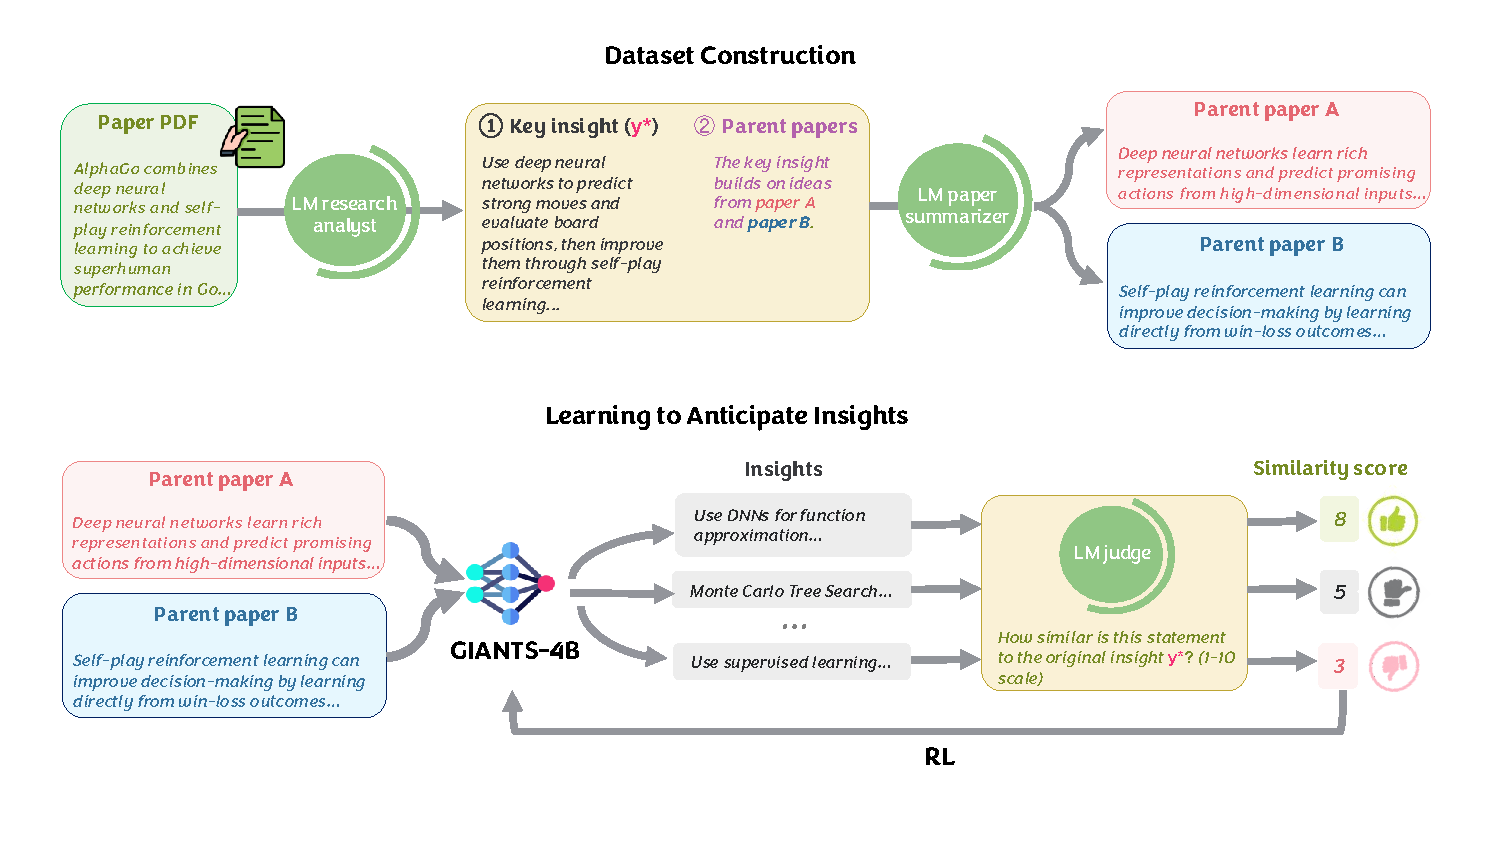
\includegraphics[width=\linewidth]{figs/giants_fig1.pdf}
    \vspace{-3mm}
    \caption{\footnotesize \textbf{Overview of \ourbenchmark{} and \ourmethod{}.} \textit{(top)} For dataset construction, we use an LM as a research analyst to process each paper PDF to identify two parent papers whose ideas are synergistically combined to produce the paper's key insight, which is extracted as the ground-truth target $y^*$. A second LM summarizes each parent paper. \textit{(bottom)} Given the two parent summaries, the model generates candidate insights, which an LM judge scores by similarity to $y^*$ on a 1–10 scale. These scores serve as a proxy reward for RL training, teaching the model to anticipate insights that more closely match real downstream papers.}
    \label{fig:giants_fig1}
    \vspace{-3mm}
\end{figure}

To evaluate insight anticipation models, we develop \ourbenchmark{}, a large-scale benchmark designed to evaluate the ability of models to synthesize two prior papers and derive the core insight of a downstream paper that builds on them (Figure~\ref{fig:giants_fig1}, top). Unlike previous benchmarks that evaluate the ability of models to answer literature synthesis questions by identifying relevant papers and generating long-form responses with citations \citep{asai2026synthesizing}, \ourbenchmark{} assesses whether a model can combine two parent papers synergistically to derive insights that lead to a subsequent paper. \ourbenchmark{} comprises $17k$ input pairs of parent paper summaries and their corresponding downstream research insights, drawn from Computer Science, Economics, Electrical Engineering, Mathematics, Physics, Quantitative Biology, Quantitative Finance, and Statistics. We also introduce an automatic evaluation method that uses an LM judge to give a \textbf{similarity score} comparing the model-generated insight to the ground-truth insight. We conducted expert evaluations of the LM judge and found that LM scores and human scores are positively correlated (Spearman's $\rho = 0.761$, $p < 0.001$).

Furthermore, we introduce \ourmethod{}, a language model trained to generate the core insight of a future scientific paper given a set of prior papers via reinforcement learning (RL). By fine-tuning with GRPO \citep{shao2024deepseekmath} to maximize the similarity scores on the research insights, the model learns to reason about connections between the input papers and generate insights that are more similar to those from real downstream papers (Figure~\ref{fig:giants_fig1}, bottom). This outperforms simply distilling the expert insight (even with reasoning traces).

We evaluate proprietary and open LMs (e.g., \gemtwopro{}, \gemthreepro{}, \qwenfourb{})
on \ourbenchmark{}. \qwenfourb{} performs similarly as \gemtwopro{} and \gemthreepro{}, despite being a smaller open model, which shows that LMs are not simply getting better at insight anticipation via scaling. In contrast, our \ourmethod{}, which uses RL with similarity scores from the LM judge as a proxy reward, significantly improves insight anticipation. 

We summarize our main contributions as follows:
\begin{itemize}
    \item \textbf{Novel paradigm for automated discovery}: We introduce the task of \emph{insight anticipation}, which isolates the creative synthesis phase of scientific progress by evaluating how effective a model is at predicting a downstream paper's core insight conditioned on foundational parent papers.
    \item \textbf{\ourbenchmark{} and evaluation metric}: We source a dataset of 17k tuples of parent and downstream papers from arXiv across eight domains and have an LM-based auto-evaluator to score the similarity between generated and ground-truth insights.
    \item \textbf{\ourmethod{}}: We present a novel approach for training a model for insight anticipation based on semantic similarity and RL, outperforming a range of proprietary and open LMs such as \gemthreepro{}.
\end{itemize}


% \footnote{\href{https://docs.cloud.google.com/vertex-ai/generative-ai/docs/models/gemini/2-5-pro}{https://docs.cloud.google.com/vertex-ai/generative-ai/docs/models/gemini/2-5-pro}}
% \footnote{\href{https://docs.cloud.google.com/vertex-ai/generative-ai/docs/models/gemini/3-pro}{https://docs.cloud.google.com/vertex-ai/generative-ai/docs/models/gemini/3-pro}}
% \footnote{\href{https://huggingface.co/Qwen/Qwen3-4B}{https://huggingface.co/Qwen/Qwen3-4B}}
% This formulation serves as a stepping stone toward the broader goal of predicting future research directions.



